\section{Monte Carlo Variance Reduction}
\label{sec:MCvar}

Monte Carlo methods for radiation transport are used in the nuclear
engineering community for a wide spectrum of application problems. Without any
variance reduction techniques, Monte Carlo methods aim to emulate
the transport of a particle from birth, through physical interaction, to death
by randomly sampling probabilities particle production, elastic and inelastic
scattering, and absorption for that particle.
This process of transporting a single particle
is repeated millions of times, which is analogous to transporting
millions of particles throughout the problem. When the user achieves a
sufficient
number of particles to sample to reach the desired statistical precision for
the region of interest, the
simulation will be complete. However, this naive approach to simulating each
particle, no matter whether it is likely to contribute to the tallied result,
can be extraordinarily computationally inefficient depending on the problem. A
user could waste time simulating millions of unusable particles and still not
reach the desired statistical precision for the tally. Variance
reduction techniques were developed to address this issue. In general, these
techniques bias the Monte Carlo transport to more effectively
contribute to a particular result, while not fundamentally changing the nature
of the problem being solved.

\subsection{Statistical Background}
\label{subsec:StatBkgnd}

Variance reduction techniques are rooted in statistics, so we will begin our
discussion of variance reduction techniques with a brief primer on the
statistical background relevant to Monte Carlo radiation transport. Monte Carlo
methods transports many randomly sampled
particles, and when those particles reach a region of interest, they are scored
in a tally. The statistical precision of the tally
will reflect the total number of particles that were sampled in- or at- this
region or surface.
The reliability of the answer obtained in this region is then dependent
on the quantity of these particles,
and the amount of time taken to move the particles on
their respective random walks through space to the region.

\subsubsection{Population Statistics}

Estimate of the variance:
\begin{equation}
S^{ 2 }=\sum _{ i=1 }^{ N }{ \frac { (x_{ i }-\bar { x } )^{ 2 } }{ N-1 }  }
             \cong \bar{x^2}-\bar{x}^2
\label{eq:Var}
\end{equation}

The variance of the mean value, or variance of $\bar{x}$, follows as:
\begin{equation}
S^{ 2 }_{ \bar { x }  }=\frac{S^2}{N}
\label{eq:VarMean}
\end{equation}

From \ref{eq:VarMean}, one can see that relationship between variance and N follows:
\begin{equation}
S_{ \bar { x }  }=\sqrt { \frac { S^{ 2 } }{ N }  } =\frac { S }{ \sqrt { N }  }
\label{eq:VarN}
\end{equation}

The relative error normalizes the variance by the mean value.
\begin{equation}
R = \frac{S_{ \bar { x }  }}{\bar{x}}
\label{eq:RelativeErr}
\end{equation}

S to R relation
\begin{equation}
S^2\:\propto\: R^2\:\propto\:\frac{1}{N}
\label{eq:S to R}
\end{equation}

\subsubsection{The Central Limit Theorem}

The central limit theorem states that:

Put central limit equation here

Mention law of large numbers

The central limit tells us that the sample mean follows a normal
distribution, regardless of the distribution of the underlying sample. This
means that no matter what distribution is being sampled, the sampled mean will
have this expected behavior. As a result, we know that the estimate of the mean,
the standard deviation, and the variance of the distribution will follow
statistics associated with a normal distribution.

\subsubsection{The Figure of Merit}

The equations in the preceeding sections describe how to estimate the statistics
of a population given a finite number of samples. In Monte Carlo radiation transport, a
user seeks to estimate some response, the relative error associated with that
response solution, and time that it takes to obtain those values.

ADD DERIVATION OF FOM HERE

The figure of merit (FOM) \eqref{eq:FOM}
is the relationship between the relative error and the
transport time. Because it describes the relationship between these two
parameters, it is often used as a success metric for variance
reduction techniques.

\begin{equation}
FOM=\frac { 1 }{ R^{ 2 }T }
\label{eq:FOM}
\end{equation}

\subsection{Variance Reduction Methods for Monte Carlo Radiation Transport}
\label{subsec:MCVR}
MCNP \cite{hendricks_mcnp_1985, brown_mcnp_2002} has a number of techniques for
variance
reduction that are accessible to users. These variance reduction
techniques fall
into four general categories: truncation methods, population control methods, modified
sampling methods, and partially-deterministic methods. Of importance for this
project are
population control methods and modified sampling methods, which are discussed in
a number
of the papers referenced herein. Truncation methods and partially-deterministic
methods do not contribute to and are not the focus of this work,
so will only be touched upon briefly. Note that while this
discussion will tend to focus towards the variance reduction methods in MCNP,
these
methods are by no means limited to this single software package. A
number of other Monte Carlo radiation transport packages also include these
methods.

Population control methods adjust the particle population in the problem to
obtain better sampling in regions of interest by preferentially increasing or
decreasing the particle population.
The first two types of population control methods that will be discussed
are called splitting and rouletting.
Splitting is a method by which the particle population can be increased by
splitting a single higher-weight particle into several lower-weight particles.
Rouletting, conversely, reduces the particle population by stochastically
killing particles. Particles that survive a rouletting routine have their weight
adjusted higher, thereby conserving weight in the routine.
Both splitting and roulette maintain a
fair game by adjusting the particle weights as splitting and rouletting are
performed; the sum of the child particle weights is the same as the parent
weight as it entered the routine.
To use population control methods effectively as a variance reduction technique,
splitting is performed in high-importance regions to increase the particle
count, and thus the sampling, in important regions. Conversely, roulette is
performed in
 low-importance
  regions to reduce the particle population in regions that are unimportant to
  the tally result.
Splitting and roulette can be applied to include geometry, energy and time,
  as well as a weight cutoff.

Rouletting and splitting can be combined in a
single method, generally referred to as weight windows. Figure \ref{fig:ww-mcnp}
illustrates the different processes a particle may go through when entering a
weight window.
%
\begin{figure}
  \centering
  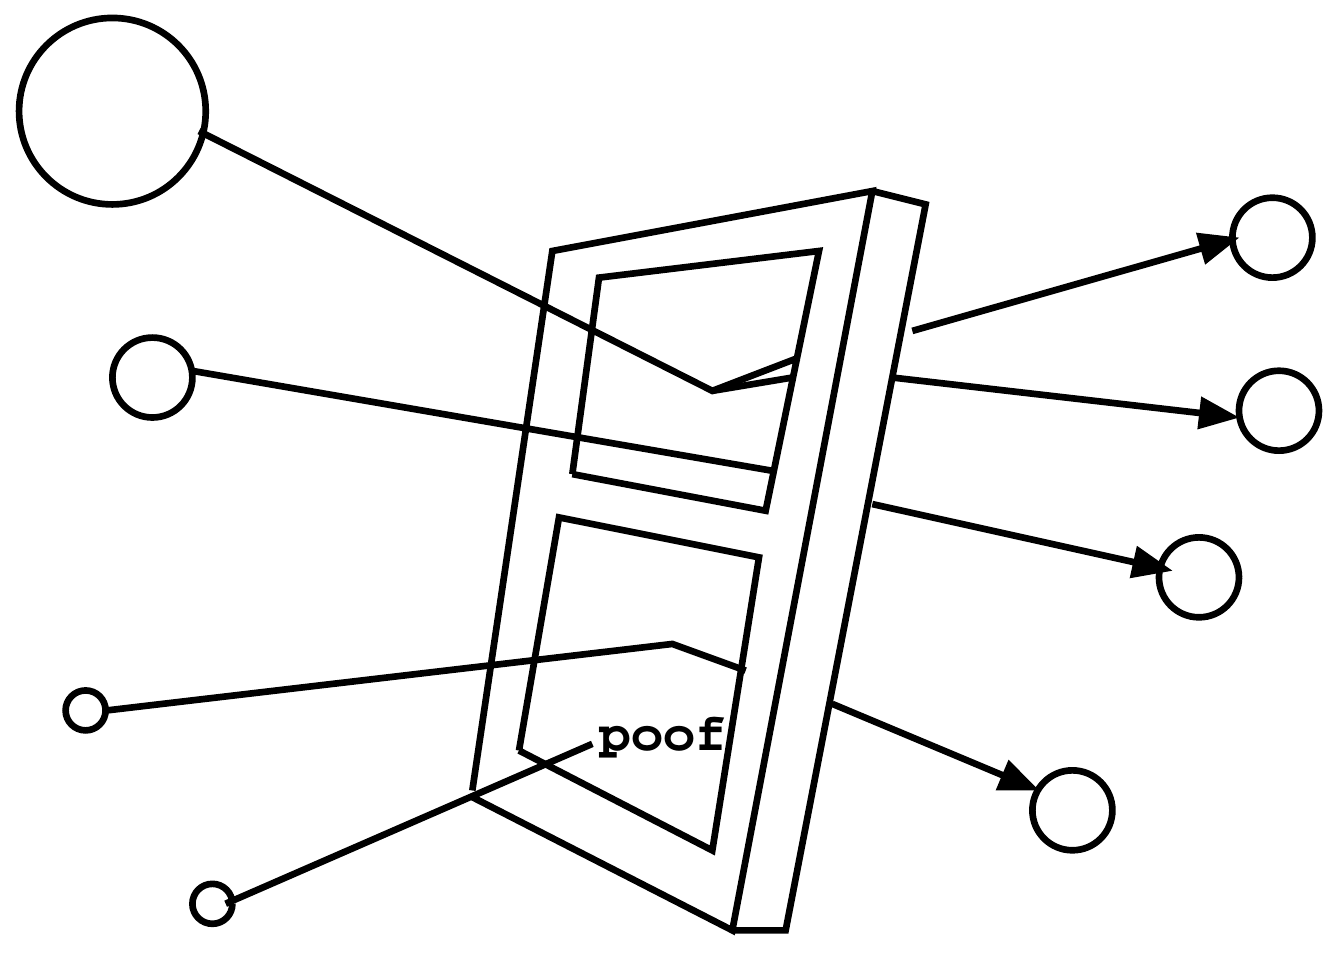
\includegraphics[width=0.5\textwidth]{./chapters/lit_review/ww-mcnp.png}
  \caption[Weight window illustration]{Cartoon illustration of a weight window,
    adapted from \cite{brown_mcnp_2002}}
  \label{fig:ww-mcnp}
\end{figure}
%
The first particle we see entering the weight window is a single, high-weight
particle. The weight of this particle is above the weight window bounds, so as
it enters the weight window it is split into multiple particles whose weight is
within the window bounds. The second particle entering the window is within the
weight window bounds, so it retains its weight and is not split or rouletted.
The last two particles entering the window have weights lower than the bound.
They undergo a rouletting routine and one particle is killed and the surviving
particle is increased in weight. As these particles leave the window, all of
them have weights within the range of the window. This will reduce the variance
of the particles contributing to a tally in that region. However, the user is
faced with calculating a significant number of parameters to
determine weight windows for the entire problem. In the best case with an
experienced user, this may just take time. With an inexperienced user or a
difficult problem this can
be insurmountable, and may be too difficult to do without some automated
assistance.

It should be noted that
while splitting and roulette can be performed on a single variable--energy,
space, or time--the weight window is either energy-space
dependent or space-time dependent. Further, the weight window will split or
roulette depending on the particle weight entering the window. Splitting and
roulette on their own either increase or decrease the particle weight
proportional to $I'/I$ no matter what the entering particle weight is. As a
result, poorly chosen splitting or roulette parameters on their own can still
have significant tally variance, because particle weights may still span a wide
range.

Modified sampling methods adjust transport by sampling from a different probability
distribution function than the actual distribution for the problem. This is
possible if, as with population control methods, the particle weights are adjusted
 accordingly.
 The new probability distribution function should bias particles in regions of high
 importance to the problem tallies. In MCNP, a number of modified sampling
 methods exist.
 These include the exponential transform, implicit capture, forced collisions, source
 biasing, and neutron-induced photon production biasing.

The exponential transform modifies particle transport from the analog problem by
artificially modifying the macroscopic cross section, and thus the
distrance-to-collision, to move particles in important directions. In directions
of higher importance, the cross section is reduced, and particles can flow more
freely. In directions of lower importance, the cross section is increased, and
particles more frequently interact, thereby increasing their probability of
directional change or absorption. The transformed cross section used by the
exponential transform is defined by
%
\begin{equation*}
  \Sigma_t^* = \Sigma_t(1-p\mu) ,
\end{equation*}
%
where $\Sigma_t^*$ is the transformed total cross section, $\Sigma_t$ is the
true total cross section, $p$ is the transform parameter, and $\mu$ is the
cosine of the angle between the preferred direction and the particle's transport
direction [MCNP MANUAL CITATION] \cite{hendricks_mcnp_1985}.

Because the particle's transport is adjusted in the exponential transform, the
particle weight must be adjusted accordingly. This is given by
%
\begin{equation*}
  \begin{split}
  w^* &= \frac{\Sigma_t e^{-\Sigma_t s}}{\Sigma_t^* e^{-\Sigma_t^* s}} \\
      &= \frac{e^{-\rho \Sigma_t \mu s}}{1-p\mu}, \\
  \end{split}
\end{equation*}
%
where $s$ is the phase space of particle residence. This weight adjustment
ensures that the particle weight is conserved throughout transport, even as
the cross section is altered. Because the cross section in the problem is both
energy and material dependent (depending on the geometry), the exponential
transform will be dependent on space and energy, and particles will be biased in
both. While a powerful method, the exponential transform is quite difficult to
use and if $p$ is chosen poorly, this method can perform quite poorly. Further,
the user has to know quite a bit about the problem physics and material to choose an
optimal quantity for $p$.

Source biasing, rather than preferentially adjusting particles' directionality
by way of adjusting the cross sections, biases particles from their origin.
Source biasing has the option to bias particles in energy, direction, and space
(if the source is volumetric). This allows the user to choose importance
separately for each variable. First, the source variable (let us consider
energy for the moment) is defined as a series of bins or a function. Second, the bins are
assigned probabilities of occurence according to their importance. An energy bin
with a high importance will be assigned a high probability of occurence, and a
bin with low importance will be assigned a low probability of occurence. As
particles are born in the bins with higher importances, they will have their
weights adjusted to the inverse of their probability of occurence, or $w^* =
p/p^*$. Here $p$ refers to the probability density function for the source
particles; it bears no relation to the exponential transform factor.

Source biasing is a very simple method that can reduce the solution variance
significantly. However, if a user chooses bin sizes or a function that does not
properly reflect the particles importances in the problem, the source will be
poorly sampled. As a result, sampling may be very inefficient and the figure of
merit will decrease. In MCNP, if poor parameters are chosen for this method, the
user will be given a warning.

Truncation methods stop tracking particles in a region of phase-space that is of
low-importance to the tally. These methods can be used in space (a vacuum boundary
condition), energy (eliminate particles above or below a specified energy), or
time (stop
tracking after a given time). To effectively use these methods, the user must be
aware of
particles' importance to a tally result. If particles that are important to a
result are
 eliminated with a truncation method, the tally will lack the contribution from
 that particle's phase-space, and will be underestimated as a result.

It is important, in using any variance reduction technique, to ensure that a
fair game
is being played. The user must ensure that the fundamental nature of the problem
is not
being changed by using a variance reduction technique, or the answer will not be
representative of the original problem. Automated variance reduction techniques aim to
eliminate this uncertainty for the user by estimating the importance of
particles in some
 way and then setting up variance reduction parameters automatically.
The remainder of this literature review will focus on efforts to
automate population
control methods and modified sampling methods for variance reduction.

\subsection{Automated Variance Reduction Methods for Monte Carlo Radiation
Transport}
\label{subsec:AutomatedMCVR}

A number of methods have automated some aspect of variance
reduction for
Monte Carlo. Some of these methods used a fast, low-particle Monte Carlo
transport run to gain an initial estimate for a cell's importance and generate
variance reduction parameters from them to bias a more computationally-intensive
run. Naturally, the variance reduction parameters generated by utilizing this
technique are limited by the statistical uncertainty in the regions used to
generate them. Furthermore, for deep-penetration particle transport, the
variance reduction parameters for low flux regions were exceedingly difficult to
generate.

As with any variance reduction technique, the goal to be achieved is a faster
time to achieve a solution for a desired uncertainty, and to reduce the variance
for the tally.
Thus the metrics for success are often the figure of merit (FOM) and the
variance for the tally obtaining the solution.
